\cotefile{148}
\scanpage{20}

\figure{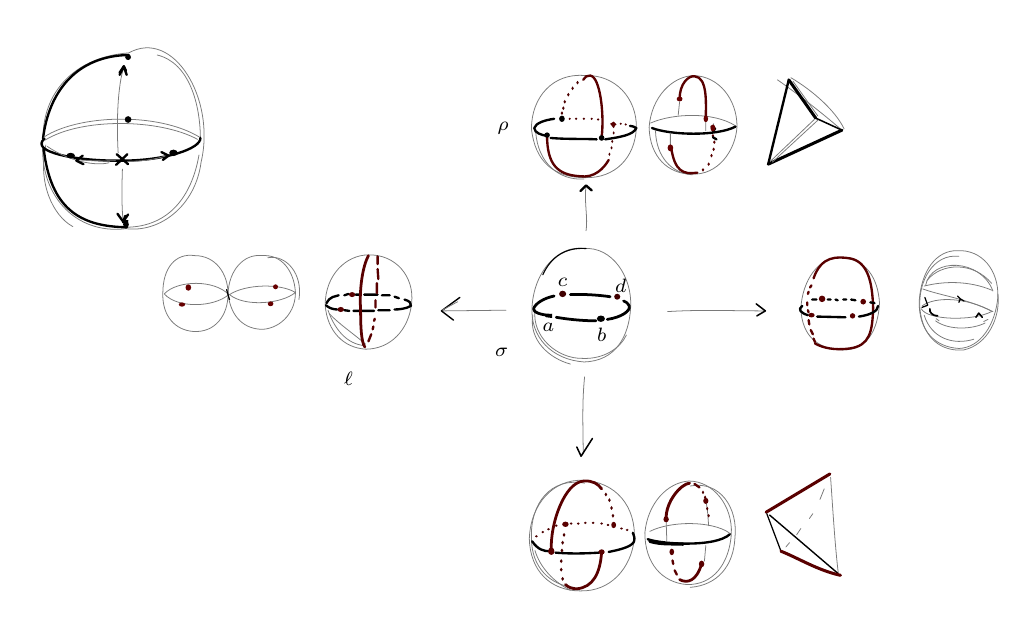
\begin{tikzpicture}[x=.009cm,y=-.009cm,line cap=round,line join=round,p/.style={draw=black!52,line width=.28pt},b/.style={draw=black,line width=.85pt},r/.style={draw=red!35!black,line width=.85pt},font=\scriptsize]
% Isolated drawing.
\draw[p] (258,88)..controls(321,53)and(381,153)..(360,242)..controls(352,304)and(302,342)..(254,336)..controls(181,345)and(130,286)..(137,210)..controls(136,145)and(180,94)..(258,88);
\draw[p] (141,218)..controls(129,271)and(151,318)..(179,333);
\draw[p] (359,210)..controls(359,162)and(344,102)..(298,91);
\draw[b] (258,91)..controls(185,92)and(145,142)..(137,209);
\draw[b] (138,224)..controls(148,307)and(188,333)..(255,334);
\draw[p] (255,334)..controls(315,333)and(347,290)..(357,232);
\draw[p] (138,207)..controls(186,175)and(299,171)..(358,207);
\draw[p] (140,211)..controls(192,179)and(302,181)..(355,210);
\draw[b] (139,209)..controls(117,228)and(185,241)..(249,240)..controls(310,240)and(360,223)..(359,208);
\draw[p] (143,220)..controls(174,241)and(211,248)..(230,243);
\draw[p] (243,229)..controls(241,197)and(241,143)..(250,111);
\draw[b] (245,119)--(251,107)--(255,119);
\draw[b] (245,116)--(251,107)--(254,113);
\draw[p] (249,252)..controls(248,279)and(248,309)..(250,324);
\draw[b] (242,315)--(250,326)--(257,316);
\draw[b] (253,318)--(250,327)--(256,325);
\draw[p] (239,240)..controls(220,241)and(203,240)..(187,239);
\draw[b] (193,233)--(184,240)--(194,245);
\draw[p] (258,241)..controls(280,241)and(300,237)..(311,233);
\draw[b] (304,228)--(314,233)--(306,239);
\draw[b] (241,231)--(257,245) (240,246)--(256,231);
\fill (257,94) circle (4.1);
\fill (257,182) circle (4.7);
\fill (176,233) ellipse (6 and 4);
\fill (321,229) ellipse (6 and 4.5);
\fill (254,330) ellipse (4 and 6);
% Upper branch.
\node at (786,194) {$\rho$};
\draw[p] (903,339)..controls(906,322)and(900,296)..(903,276);
\draw[b] (895,283)--(903,275)--(911,282);
\draw[p] (901,120)..controls(857,116)and(826,150)..(826,195)..controls(831,241)and(857,264)..(902,264)..controls(944,265)and(972,236)..(974,194)..controls(975,152)and(944,118)..(901,120);
\draw[p] (832,199)..controls(835,244)and(865,268)..(900,266);
\draw[b] (858,181)..controls(844,183)and(832,187)..(830,194)..controls(830,201)and(841,204)..(847,205);
\draw[b] (853,208)..controls(874,210)and(902,209)..(918,210);
\draw[b] (930,210)..controls(950,207)and(970,204)..(974,194)..controls(971,192)and(967,191)..(965,191);
\foreach \x/\y in {880/181,889/181,900/181,911/181,920/182,952/188,959/189}{\fill[red!30!black] (\x,\y) circle (1.7);}
\draw[r] (848,204)..controls(848,246)and(863,260)..(894,262)..controls(915,265)and(928,251)..(935,239);
\foreach \x/\y in {936/231,939/222,940/213,942/201,942/192}{\fill[red!30!black] (\x,\y) ellipse (1.5 and 2.3);}
\draw[r] (925,207)..controls(929,175)and(923,122)..(909,120)..controls(905,119)and(901,122)..(899,126);
\foreach \x/\y in {891/130,884/138,878/147,873/157,871/166,869/173}{\fill[red!30!black] (\x,\y) ellipse (1.8 and 2.6);}
\fill (848,204) ellipse (4 and 3.8);
\fill (925,208) ellipse (4 and 4);
\fill (869,181) ellipse (4 and 4.5);
\fill[red!35!black] (942,185)--(946,189)--(941,193)--(937,188)--cycle;
\draw[p] (1055,120)..controls(1024,121)and(995,151)..(992,193)..controls(993,235)and(1019,259)..(1052,259)..controls(1089,261)and(1114,226)..(1116,192)..controls(1116,153)and(1090,121)..(1055,120);
\draw[p] (1001,198)..controls(1002,235)and(1024,258)..(1053,260);
\draw[p] (994,187)..controls(1026,173)and(1083,171)..(1114,191);
\draw[b] (996,194)..controls(1022,204)and(1087,206)..(1114,192);
\draw[p] (1035,157)--(1033,176) (1072,183)--(1072,198) (1022,201)--(1022,222);
\draw[r] (1035,153)..controls(1035,132)and(1047,120)..(1056,121)..controls(1075,122)and(1072,161)..(1072,180);
\draw[r] (1023,221)..controls(1028,255)and(1040,260)..(1060,257);
\foreach \x/\y in {1068/253,1076/245,1080/233,1083/224,1084/214,1082/205}{\fill[red!35!black] (\x,\y) ellipse (1.8 and 2.5);}
\draw[b] (1082,199)--(1085,195)--(1080,192) (1082,207)--(1087,210);
\draw[p] (1083,188)--(1082,193);
\fill[red!40!black] (1035,153) ellipse (4.1 and 3.5);
\fill[red!40!black] (1072,181) ellipse (3.2 and 4.8);
\fill[red!40!black] (1022,222) ellipse (4 and 5);
\fill[red!40!black] (1082,194) ellipse (3.5 and 4.8);
\draw[p] (1173,126)..controls(1199,144)and(1235,172)..(1264,197);
\draw[p] (1192,123)..controls(1224,142)and(1255,170)..(1267,195);
\draw[b] (1189,126)--(1160,245);
\draw[b,line width=1.1pt] (1189,126)--(1227,180);
\draw[p] (1195,128)--(1230,177);
\draw[b,line width=.55pt] (1227,180)--(1264,197);
\draw[b,line width=1.1pt] (1160,245)--(1264,197);
\draw[p] (1163,241)--(1225,182);
\draw[p] (1166,242)--(1230,183);
% Left branch.
\draw[p] (351,374)..controls(324,370)and(306,391)..(306,427)..controls(305,459)and(323,479)..(349,481)..controls(380,483)and(398,458)..(398,428)..controls(398,400)and(381,374)..(351,374);
\draw[p] (446,374)..controls(420,371)and(399,395)..(398,428)..controls(402,462)and(422,478)..(447,478)..controls(474,476)and(494,452)..(493,425)..controls(491,396)and(474,372)..(446,374);
\draw[p] (454,377)..controls(480,372)and(504,400)..(498,436);
\draw[p] (308,428)..controls(327,408)and(379,408)..(399,429)..controls(378,447)and(327,449)..(308,428);
\draw[p] (400,429)..controls(423,414)and(472,413)..(493,426)..controls(474,442)and(422,447)..(400,429);
\draw[b,line width=.45pt] (396,422)--(400,436);
\fill[red!40!black] (342,419) ellipse (4 and 4.5);
\fill[red!40!black] (333,443) ellipse (4.5 and 3);
\fill[red!40!black] (465,418) circle (3.5);
\fill[red!40!black] (458,442) ellipse (4 and 3.4);
\draw[p] (596,373)..controls(565,373)and(535,401)..(535,444)..controls(538,481)and(561,504)..(592,506)..controls(627,506)and(653,479)..(657,441)..controls(661,403)and(634,372)..(596,373);
\draw[p] (539,451)..controls(548,477)and(565,499)..(591,501);
\draw[p] (541,456)..controls(555,471)and(575,484)..(592,499);
\draw[b] (537,441)..controls(542,431)and(549,432)..(554,430);
\draw[b] (562,430)--(568,428);
\draw[b] (578,429)--(585,429) (590,429)--(609,429) (615,430)--(626,430) (633,432)--(639,434);
\draw[b] (647,436)..controls(654,438)and(657,441)..(656,445)..controls(649,449)and(639,450)..(633,450);
\draw[b] (536,444)..controls(540,448)and(547,450)..(552,450);
\draw[b] (562,451)--(569,452) (575,452)--(604,452) (610,451)--(626,451);
\fill[red!35!black] (573,429) ellipse (4.5 and 3.5);
\fill[red!35!black] (557,450) ellipse (4.6 and 3.6);
\draw[r,line width=1pt] (596,374)..controls(588,389)and(583,420)..(585,451)..controls(585,475)and(586,496)..(591,503);
\draw[r] (609,375)--(609,386) (609,393)--(610,407) (608,413)--(608,427) (606,437)--(606,447);
\draw[r] (605,463)--(604,466) (603,474)--(602,478) (600,485)--(596,495);
\node at (568,548) {$\ell$};
\draw[p] (790,451)--(701,452);
\draw[b,line width=.5pt] (725,433)--(699,452)--(716,465);
\draw[p] (722,439)--(700,451);
\node at (784,511) {$\sigma$};
% Central sphere.
\draw[p] (900,364)..controls(866,359)and(831,393)..(827,444)..controls(823,490)and(856,521)..(900,524)..controls(944,523)and(964,489)..(966,446)..controls(968,404)and(940,361)..(900,364);
\draw[b,line width=.4pt] (842,401)..controls(854,375)and(875,362)..(903,364);
\draw[p] (831,452)..controls(827,488)and(862,520)..(899,519)..controls(928,520)and(951,505)..(960,486);
\draw[p] (828,458)..controls(822,493)and(851,519)..(881,527);
\draw[b,line width=1pt] (858,431)..controls(843,434)and(831,442)..(829,449)..controls(828,454)and(841,458)..(851,458);
\draw[b,line width=1pt] (861,461)..controls(884,465)and(905,466)..(917,466);
\draw[b,line width=1pt] (933,464)..controls(953,461)and(966,452)..(964,445)..controls(961,440)and(959,439)..(956,438);
\draw[b,line width=1pt] (881,429)..controls(900,428)and(924,430)..(937,432);
\fill[red!25!black] (870,428) ellipse (5 and 4.5);
\fill[red!25!black] (947,432) ellipse (4.3 and 4.2);
\fill (842,457)--(855,456)--(855,462)--(847,461)--cycle;
\fill (924,463) ellipse (5.7 and 4.5);
\node at (870,412) {$c$};
\node at (952,416) {$d$};
\node at (850,475) {$a$};
\node at (925,485) {$b$};
% Right branch.
\draw[p] (1018,453)..controls(1063,450)and(1112,452)..(1154,452);
\draw[b,line width=.55pt] (1143,442)--(1156,452)--(1144,459);
\draw[p] (1262,377)..controls(1230,376)and(1208,410)..(1206,449)..controls(1208,488)and(1230,506)..(1265,507)..controls(1300,508)and(1315,478)..(1317,441)..controls(1315,406)and(1298,378)..(1262,377);
\draw[r] (1224,406)..controls(1235,374)and(1257,375)..(1276,378)..controls(1300,383)and(1307,410)..(1308,448)..controls(1307,482)and(1303,501)..(1275,505)..controls(1253,508)and(1237,504)..(1226,498);
\draw[r] (1221,416)--(1219,419) (1217,425)--(1216,428) (1215,440)--(1215,444) (1216,451)--(1217,454) (1217,465)--(1218,471) (1220,479)--(1223,485) (1224,491)--(1226,496);
\draw[b] (1208,445)..controls(1201,450)and(1206,455)..(1216,458);
\draw[b] (1229,460)--(1269,461);
\draw[b] (1288,460)..controls(1302,458)and(1315,453)..(1315,445);
\draw[b] (1222,436)--(1228,436) (1244,436)--(1248,436) (1255,436)--(1258,437) (1266,436)--(1270,436) (1277,436)--(1283,437) (1304,440)--(1310,441);
\fill[red!35!black] (1236,435) circle (4.6);
\fill[red!35!black] (1294,439) circle (4);
\fill[red!35!black] (1221,458) ellipse (4.5 and 3.2);
\fill[red!35!black] (1279,459) circle (3.8);
\draw[p] (1426,367)..controls(1397,367)and(1376,395)..(1373,438)..controls(1372,481)and(1396,503)..(1429,505)..controls(1460,504)and(1481,470)..(1484,432)..controls(1485,395)and(1462,365)..(1426,367);
\draw[p] (1429,375)..controls(1393,371)and(1371,410)..(1374,449)..controls(1378,491)and(1405,510)..(1436,507)..controls(1469,500)and(1488,462)..(1484,428);
\draw[p] (1382,416)..controls(1390,376)and(1460,378)..(1477,424);
\draw[p] (1384,409)..controls(1404,384)and(1449,382)..(1475,413);
\draw[p] (1380,417)..controls(1407,410)and(1443,409)..(1476,423);
\draw[p] (1378,421)..controls(1402,430)and(1441,435)..(1477,453);
\draw[p] (1377,445)..controls(1396,431)and(1441,433)..(1476,453);
\draw[p] (1376,449)..controls(1384,465)and(1448,467)..(1475,453);
\draw[p] (1396,466)..controls(1415,480)and(1449,478)..(1466,469);
\draw[p] (1380,458)..controls(1390,490)and(1420,501)..(1450,492);
\draw[b,line width=.45pt] (1381,433)--(1385,444)--(1377,447);
\draw[b,line width=.45pt] (1427,431)--(1431,435)--(1429,440) (1431,435)--(1436,438);
\draw[b,line width=.6pt] (1388,449)..controls(1387,454)and(1392,459)..(1399,459);
\draw[b,line width=.55pt] (1453,461)--(1457,455)--(1462,461);
\draw[p] (1397,463)--(1401,466) (1464,467)--(1470,464);
% Lower branch.
\draw[p] (901,545)..controls(897,583)and(899,620)..(899,654);
\draw[b,line width=.55pt] (890,644)--(896,657)--(912,632);
\draw[p] (899,691)..controls(857,689)and(825,724)..(823,773)..controls(824,819)and(853,847)..(895,847)..controls(938,848)and(966,815)..(971,775)..controls(974,728)and(945,693)..(899,691);
\draw[p] (901,695)..controls(853,686)and(824,724)..(826,773)..controls(826,813)and(852,839)..(886,842);
\draw[p] (831,790)..controls(838,814)and(858,835)..(881,846);
\draw[b] (827,777)..controls(835,789)and(844,791)..(851,791);
\draw[b] (860,793)..controls(883,795)and(907,794)..(921,793);
\draw[b] (935,792)..controls(956,788)and(970,783)..(971,776)..controls(972,771)and(970,768)..(969,765);
\foreach \x/\y in {833/770,842/764,850/760,861/755,882/752,892/752,902/751,913/751,925/752,934/754,953/759,961/761}{\fill[red!30!black] (\x,\y) ellipse (2 and 1.7);}
\draw[r,line width=1pt] (854,791)..controls(852,752)and(873,693)..(900,692)..controls(912,691)and(920,696)..(925,703);
\foreach \x/\y in {931/711,936/719,939/730,941/741}{\fill[red!30!black] (\x,\y) ellipse (1.9 and 2.8);}
\draw[r,line width=1pt] (925,792)..controls(923,822)and(913,842)..(890,844)..controls(883,844)and(878,842)..(874,838);
\foreach \x/\y in {870/830,868/817,868/805,869/790,870/779,872/768}{\fill[red!30!black] (\x,\y) ellipse (2 and 2.8);}
\fill[red!35!black] (854,791) ellipse (4.5 and 5.3);
\fill[red!35!black] (925,792) ellipse (4.3 and 3.7);
\fill[red!35!black] (874,753) ellipse (4.6 and 3.8);
\fill[red!35!black] (942,754) ellipse (3.4 and 4.5);
\draw[p] (1048,692)..controls(1018,694)and(990,723)..(986,765)..controls(986,808)and(1010,835)..(1045,838)..controls(1083,839)and(1105,808)..(1108,767)..controls(1110,726)and(1082,692)..(1048,692);
\draw[p] (1050,699)..controls(1092,691)and(1118,730)..(1113,773)..controls(1111,811)and(1089,839)..(1050,842);
\draw[p] (993,763)..controls(1023,748)and(1080,748)..(1105,765);
\draw[b] (990,774)..controls(1009,781)and(1086,786)..(1106,767);
\draw[b,line width=1.2pt] (993,777)..controls(1010,782)and(1027,780)..(1040,781);
\draw[p] (1016,748)--(1017,777) (1072,720)..controls(1075,734)and(1075,745)..(1076,755) (1072,783)--(1070,805);
\draw[r,line width=1.05pt] (1016,746)..controls(1015,721)and(1037,696)..(1049,695);
\draw[r] (1056,696)--(1063,701);
\foreach \x/\y in {1068/708,1071/715,1074/731,1076/741}{\fill[red!30!black] (\x,\y) ellipse (1.7 and 2.6);}
\draw[r,line width=1pt] (1066,809)..controls(1059,833)and(1046,837)..(1035,831);
\draw[r] (1031,824)--(1028,818) (1026,809)--(1025,804);
\fill[red!35!black] (1016,746) ellipse (3.8 and 4.2);
\fill[red!35!black] (1072,720) ellipse (3.7 and 4.3);
\fill[red!35!black] (1024,792) ellipse (3.3 and 4.6);
\fill[red!35!black] (1066,809) ellipse (3.8 and 4.7);
\draw[r,line width=1.1pt] (1157,736)--(1247,682);
\draw[p] (1248,687)..controls(1251,729)and(1254,782)..(1259,823);
\draw[b,line width=.45pt] (1158,738)--(1178,791);
\draw[b,line width=.5pt] (1162,740)--(1258,822);
\draw[r,line width=1.1pt] (1178,791)..controls(1203,801)and(1230,818)..(1262,825);
\draw[p] (1185,785)--(1190,779) (1200,768)--(1206,759) (1218,745)--(1223,738) (1233,718)--(1239,703);
\end{tikzpicture}}

% FORMULAS
\[
\begin{aligned}
I&\unsure{=|\simeq}\unsure{S_Q|I_Q}=\coprod_{d\in D_Q}d\\
A_Q&=\prod_{d\in D_Q}d\\
C_Q&=\bigwedge_{d\in D_Q}d=\perp\\
\omega_Q&=C_Q\wedge D_Q\\
\omega_I&\simeq\omega_J\simeq C_Q\simeq J\setminus\{Q\}
\end{aligned}
\]

% PARTITIONS
\figure{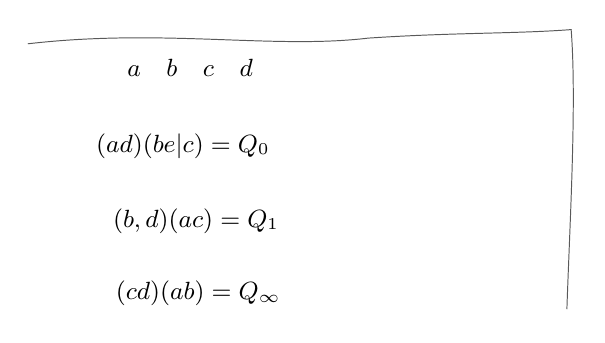
\begin{tikzpicture}[x=.018cm,y=-.018cm,line cap=round,line join=round,font=\small]
\draw[black!65,line width=.35pt] (80,997)..controls(175,986)and(253,1001)..(320,993)..controls(380,989)and(424,990)..(463,987);
\draw[black!65,line width=.35pt] (463,987)..controls(467,1038)and(462,1124)..(460,1184);
\node[anchor=west] at (143,1014) {$a\quad b\quad c\quad d$};
\node[anchor=west] at (121,1069) {$(ad)(b\unsure{e|c})=Q_0$};
\node[anchor=west] at (133,1122) {$(b,d)(ac)=Q_1$};
\node[anchor=west] at (135,1173) {$(cd)(ab)=Q_\infty$};
\end{tikzpicture}}

% EQUIVALENCE
\figure{\begin{tikzpicture}[x=.014cm,y=-.014cm,line cap=round,line join=round,font=\small]
% Weak upper pencil annotation.
\node[anchor=west,text=black!50,scale=.85,inner sep=0pt] at (858,992) {\unsure{tétraèdre $+$ b}};
\node[anchor=west,inner sep=0pt] at (1080,982) {\unsure{\begin{tikzpicture}[x=.018cm,y=-.018cm,baseline=-.5ex,line cap=round,line join=round]
\draw[black!45,line width=.3pt] (1,18)..controls(10,13)and(11,20)..(17,19);
\draw[black!45,line width=.3pt] (20,17)..controls(25,23)and(28,27)..(31,25);
\draw[black!45,line width=.3pt] (39,8)--(34,28);
\draw[black!45,line width=.3pt] (47,17)..controls(55,13)and(59,17)..(63,16);
\draw[black!45,line width=.3pt] (53,24)--(67,22);
\end{tikzpicture}}};
\node[anchor=west,text=black!50,scale=.85,inner sep=0pt] at (1193,995) {\unsure{(carré $+$}};
% Live expression and raised word.
\node[anchor=west,inner sep=0pt] at (570,1044) {(tétraèdre $+$ diagonale)};
\node[anchor=west,inner sep=0pt] at (1059,1041) {(carré $+$ codiagonale)};
\node[anchor=south,inner sep=0pt] at (709,1024) {\inserted{orienté}};
\draw[line width=.55pt] (657,1020)..controls(680,1027)and(746,1025)..(770,1017);
\draw[line width=.55pt] (713,1025)--(716,1038);
\draw[line width=1pt] (963,1038)--(1053,1037);
\draw[line width=.9pt] (978,1023)--(961,1038)--(978,1050);
\draw[line width=.9pt] (1038,1024)--(1055,1037)--(1040,1051);
% First faint line below the left term, with its intersecting leading strokes.
\node[anchor=north west,inner sep=0pt] at (631,1063) {\unsure{
\begin{tikzpicture}[x=.014cm,y=-.014cm,baseline=-.5ex,line cap=round,line join=round]
\draw[black!50,line width=.32pt] (17,3)..controls(18,11)and(21,20)..(20,29);
\draw[black!50,line width=.32pt] (1,27)--(39,22);
\draw[black!50,line width=.32pt] (7,32)..controls(19,24)and(27,12)..(34,3);
\draw[black!50,line width=.32pt] (18,20)--(43,31);
\draw[black!50,line width=.32pt] (57,10)..controls(52,22)and(50,34)..(57,34)..controls(64,32)and(66,24)..(67,19)..controls(65,35)and(77,33)..(79,18);
\draw[black!50,line width=.32pt] (82,32)--(98,33) (89,33)--(90,46) (83,46)--(99,45);
\draw[black!50,line width=.32pt] (113,18)--(132,35) (115,36)--(131,18);
\draw[black!50,line width=.32pt] (156,14)..controls(158,24)and(161,30)..(169,33)..controls(158,35)and(151,33)..(146,32);
\end{tikzpicture}}};
% Further faint formula line: exact contents remain undecided.
\node[anchor=north west,inner sep=0pt] at (682,1117) {\unsure{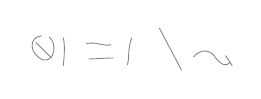
\begin{tikzpicture}[x=.014cm,y=-.014cm,baseline=-.5ex,line cap=round,line join=round]
\draw[black!48,line width=.32pt] (17,8)..controls(5,9)and(6,25)..(19,30)..controls(30,31)and(31,14)..(24,9);
\draw[black!48,line width=.32pt] (12,14)--(26,28);
\draw[black!48,line width=.32pt] (37,10)..controls(39,20)and(37,31)..(37,35);
\draw[black!48,line width=.32pt] (58,15)..controls(68,13)and(73,18)..(80,16);
\draw[black!48,line width=.32pt] (60,29)--(82,28);
\draw[black!48,line width=.32pt] (99,10)..controls(95,19)and(97,29)..(95,34);
\draw[black!48,line width=.32pt] (124,1)--(144,39);
\draw[black!48,line width=.32pt] (155,27)..controls(163,18)and(172,22)..(175,28)..controls(181,35)and(185,36)..(188,32);
\draw[black!48,line width=.32pt] (184,26)--(190,35);
\end{tikzpicture}}};
% Brace below the central span and its two formula baselines.
\draw[line width=.55pt] (884,1085)..controls(882,1096)and(895,1101)..(923,1102)..controls(955,1103)and(979,1116)..(993,1129)..controls(1005,1115)and(1022,1101)..(1050,1104)..controls(1082,1108)and(1106,1104)..(1110,1095);
\node[anchor=west,inner sep=0pt] at (941,1162) {$\omega_I\times J$};
\node[anchor=west,inner sep=0pt] at (915,1215) {$\simeq J\times\omega_I$};
\end{tikzpicture}}

% EXACT_SEQUENCE
\diagram{\begin{tikzcd}
0\arrow[r]&V(J)\arrow[r]&\unsure{\mathfrak S}_I\arrow[r]&\unsure{\mathfrak S}_J\arrow[r]&1
\end{tikzcd}}

% PENCIL_SHAPE
\figure{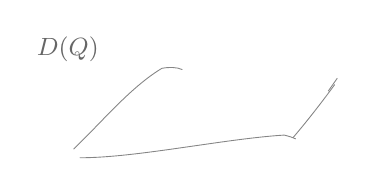
\begin{tikzpicture}[x=.016cm,y=-.016cm,line cap=round,line join=round,font=\small]
\node[anchor=west,text=black!60] at (195,1372) {$\unsure{D(Q)}$};
\draw[black!48,line width=.32pt] (232,1451)..controls(254,1430)and(277,1402)..(302,1387)..controls(307,1386)and(314,1386)..(318,1388);
\draw[black!48,line width=.32pt] (237,1458)..controls(282,1458)and(351,1443)..(399,1440)..controls(403,1441)and(406,1442)..(408,1443);
\draw[black!48,line width=.32pt] (406,1442)..controls(418,1428)and(431,1411)..(439,1400);
\draw[black!48,line width=.32pt] (434,1405)--(441,1395);
\end{tikzpicture}}

% RELATIONS
\figure{\begin{tikzpicture}[x=.015cm,y=-.015cm,line cap=round,line join=round,font=\large]
\draw[black!58,line width=.35pt] (732,1298)..controls(867,1292)and(1024,1271)..(1167,1279);
\draw[black!58,line width=.35pt] (1167,1282)..controls(1168,1372)and(1166,1483)..(1174,1549);
\draw[black!58,line width=.35pt] (711,1341)..controls(714,1423)and(713,1510)..(720,1571);
\draw[black!58,line width=.35pt] (728,1570)..controls(858,1552)and(999,1564)..(1105,1558)..controls(1109,1558)and(1111,1560)..(1113,1561);
\node[anchor=west] at (773,1418) {$\left\{\begin{aligned}\rho^3&=\sigma^2=1\\[1.1ex]\rho\sigma&=\ell\end{aligned}\right.$};
\end{tikzpicture}}

% LOWER_DIAGRAM
% Lower array: the faint overlay and hatched superscript retain their actual strokes.
% A question at either graphic locus marks the unresolved character identification.
\diagram{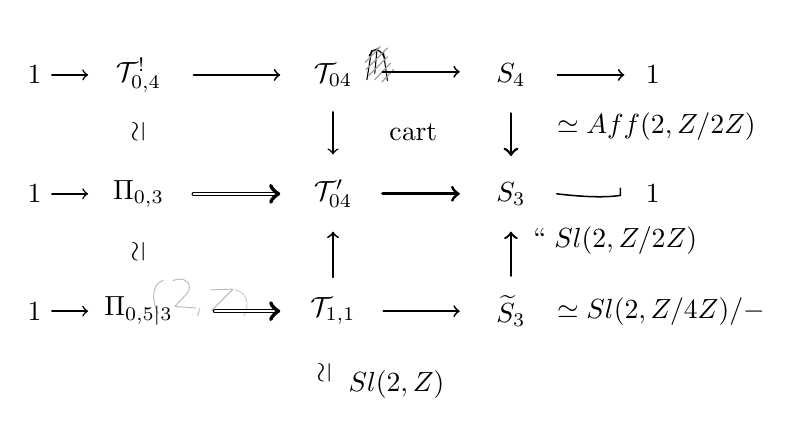
\begin{tikzpicture}[x=1cm,y=1cm,line cap=round,line join=round]
% Pale overwritten span beside the lower Pi; drawn before the dark label and shaft.
\draw[gray!55,line width=.35pt] (1.63,-2.61)..controls(1.49,-2.65)and(1.48,-2.87)..(1.57,-3.03);
\draw[gray!55,line width=.35pt] (1.76,-2.61)..controls(1.91,-2.55)and(2.02,-2.66)..(1.94,-2.77)--(1.78,-2.94)--(2.05,-2.96);
\draw[gray!50,line width=.35pt] (2.10,-2.96)--(2.07,-3.06);
\draw[gray!55,line width=.35pt] (2.24,-2.73)--(2.52,-2.72)--(2.25,-2.99)--(2.54,-2.99);
\draw[gray!45,line width=.3pt] (2.55,-2.73)..controls(2.69,-2.76)and(2.74,-2.90)..(2.66,-3.06);
\node[inner sep=0pt] at (2.79,-3.19) {$\unsure{\phantom{A}}$};
\node[inner sep=0pt] (u0) at (0,0) {$1$};
\node[inner sep=0pt] (u1) at (1.32,0) {$\mathcal T_{0,4}^{!}$};
\node[inner sep=0pt] (u2) at (3.79,0) {$\mathcal T_{04}$};
\node[inner sep=0pt] (u3) at (6.05,0) {$\unsure{\mathfrak S}_4$};
\node[inner sep=0pt] (u4) at (7.85,0) {$1$};
\node[inner sep=0pt] (m0) at (0,-1.51) {$1$};
\node[inner sep=0pt] (m1) at (1.32,-1.51) {$\Pi_{0,3}$};
\node[inner sep=0pt] (m2) at (3.79,-1.51) {$\mathcal T'_{04}$};
\node[inner sep=0pt] (m3) at (6.05,-1.51) {$\unsure{\mathfrak S}_3$};
\node[inner sep=0pt] (m4) at (7.85,-1.51) {$1$};
\node[inner sep=0pt] (l0) at (0,-3.00) {$1$};
\node[inner sep=0pt] (l1) at (1.32,-3.00) {$\Pi_{0,\unsure{5|3}}$};
\node[inner sep=0pt] (l2) at (3.79,-3.00) {$\mathcal T_{1,1}$};
\node[inner sep=0pt] (l3) at (6.05,-3.00) {$\widetilde{\unsure{\mathfrak S}}_3$};
\draw[->,line width=.55pt] (.22,0)--(.68,0);
\draw[->,line width=.65pt] (2.02,0)--(3.12,0);
% The upper middle arrow begins in the crossed raised cluster.
\draw[line width=.45pt] (4.25,.24)..controls(4.31,.39)and(4.42,.30)..(4.45,.20);
\draw[line width=.4pt] (4.28,.31)--(4.22,-.06) (4.35,.34)--(4.32,.02) (4.43,.29)--(4.48,-.07);
\draw[gray!75,line width=.45pt] (4.20,.16)--(4.39,.36) (4.21,.07)--(4.48,.34) (4.24,-.01)--(4.48,.23) (4.32,-.06)--(4.52,.15) (4.41,-.09)--(4.56,.07);
\node[inner sep=0pt] at (4.53,.48) {$\unsure{\phantom{A}}$};
\draw[->,line width=.65pt] (4.42,.04)--(5.40,.04);
\draw[->,line width=.65pt] (6.64,0)--(7.49,0);
\draw[->,line width=.55pt] (.22,-1.51)--(.68,-1.51);
\draw[double,double distance=.65pt,->,line width=.45pt] (2.02,-1.51)--(3.12,-1.51);
\draw[->,line width=1.1pt] (4.42,-1.51)--(5.40,-1.51);
% The middle terminal connector has a blunt upturned end, without a supplied head.
\draw[line width=.55pt] (6.63,-1.51)..controls(6.98,-1.55)and(7.24,-1.56)..(7.44,-1.53)--(7.44,-1.44);
\draw[->,line width=.55pt] (.22,-3.00)--(.68,-3.00);
\draw[double,double distance=.65pt,->,line width=.45pt] (2.29,-3.00)--(3.12,-3.00);
\draw[->,line width=.65pt] (4.43,-3.00)--(5.40,-3.00);
\draw[->,line width=.55pt] (3.79,-.47)--(3.79,-1.01);
\draw[->,line width=1pt] (6.05,-.49)--(6.05,-1.03);
\draw[->,line width=.65pt] (3.79,-2.57)--(3.79,-1.99);
\draw[->,line width=.85pt] (6.05,-2.55)--(6.05,-1.99);
\node[inner sep=0pt] at (1.32,-.72) {\rotatebox{90}{$\simeq$}};
\node[inner sep=0pt] at (1.32,-2.24) {\rotatebox{90}{$\simeq$}};
\node[inner sep=0pt] at (4.81,-.72) {cart};
\node[anchor=west,inner sep=0pt] at (6.63,-.65) {$\simeq\operatorname{Aff}(2,\mathbb Z/2\mathbb Z)$};
\node[anchor=west,inner sep=0pt] at (6.30,-2.10) {`` $\operatorname{Sl}(2,\mathbb Z/2\mathbb Z)$};
\node[anchor=west,inner sep=0pt] at (6.63,-3.00) {$\simeq\operatorname{Sl}(2,\mathbb Z/4\mathbb Z)/-$};
\node[inner sep=0pt] at (3.68,-3.78) {\rotatebox{90}{$\simeq$}};
\node[anchor=west,inner sep=0pt] at (3.98,-3.93) {$\operatorname{Sl}(2,\mathbb Z)$};
\end{tikzpicture}}

\margin{19}
